\documentclass[a4paper]{../phyreport}
\expName{温度传感器特性研究及测水比热}
\expDate{2024}{4}{22}
\subDate{2024}{}{}
% \expAddr{致原楼}
% 实验预习处: http://172.31.80.102:7101/
% 快乐制表网站: https://www.tablesgenerator.com/#
\usepackage{subcaption}
\usepackage{longtable}
\begin{document}
\phyExpCover

\section{实验设计方案}  
\subsection{实验目的}
\begin{enumerate}
  \item 了解Pt100铂电阻和热敏电阻NTC的温度特性及其测温原理;
  \item 学习用恒电流法和直流电桥法测量热电阻;
  \item 了解PN结正的温度特性及其测温原理;  
  \item 学习运用不同的温度传感器设计测温电路。
\end{enumerate}
\subsection{实验原理}
\subsubsection{温度传感器}

温度传感器是指能够利用物质各种物理性质随温度变化的规律把温度转换为电信号的器件或装置。
一般说来,温度传感器由敏感元件和变换元件两部分组成。

1、双金属温度计
双金属温度计是基于固体受热膨胀的原理,两种热膨胀系数差异较大的金属片粘贴在一起,将其中的一端固定,另一端作为自由端,自由端与指针相连。  

当温度变化时,因双金属片的两种不同材料线膨胀系数差异相对很大,而产生不同的膨胀和收缩,导致双金属片产生弯曲变形。温度变化越大则产生的线膨胀差越大,引起的弯曲角度也越大。自由端位移的大小与温度成一定的函数关系。

2、压力温度计
压力温度计主要由充有感温介质的感温包、传递压力元件(毛细管)及压力敏感元件齿轮或杠杆传动机构、指针和读数盘组成。

测温时将其温包置入被测介质中,温包内的感温介质(为气体或液体或蒸发液体)因被测温度的高低而导致其体积膨胀或收缩造成压力的增减,压力的变化经毛细管传给弹簧管使其产生变形,进而通过传动机构带动指针偏转,指示出相应的温度。

两种不同的金属A与B形成闭合回路,当两个接点温度不同时回路将产生电势,该电势的方向和大小取决于两导体的材料及两接点之间的温度差,而与导体的粗细、长短无关。这种现象称为热电效应,组成的测量传感器称为热电偶。

5、红外辐射测温
只要温度高于绝对零度,物体都有一定波长的电磁波辐射,热辐射温度检测就是基于这个原理实现温度测量的。
医用红外热像仪一般由:镜头、红外探测器、信号处理单元和显示部分组成。


6、光纤温度传感器——特殊场合下的测温

% 热电阻温度特性测量

\subsubsection{传感器原理}

\paragraph{Pt100} 铂电阻的阻值随温度变化而变化计算公式:
\begin{align}
  \label{eq:2}
-200<t<0 ℃ :& \quad {R_t} = {R_0}\left[ {1 + At + B{t^2} + C(t - 100^\circ C){t^3}} \right]\\
0<t<850 ℃ :& \quad R_t=R_0(1+At+Bt)^2 
\end{align}
式中$Rt,R0$分别为铂电阻在温度t、0℃时的电阻值,
A、B、C为温度系数:
$A=3.90802×10^{-3}C^{-1};B=-5.802×10^{-7}C^{-2} ;C=-4.27350×10^{-12}C^{-4}$

在$0 \sim 100$℃范围内Rt的表达式可近似线性为:

\begin{equation}
\label{eq:1}
R_t=R_0(1+A_1t)
\end{equation}
式中A1温度系数,近似为3.85×10ˉ³/℃,Pt100铂电阻的阻值, 其0℃时 $R_t =100\Omega$;而100℃时 $R_t =138.5Ω$.

\paragraph{热敏电阻}
热敏电阻是利用某种半导体材料的电阻率随温度变化而变化的性质制成的。它的电阻值随温度的变化而剧烈的变化,可以提供较大的灵敏度。\\
电阻值随温度的升高而升高的,称正温度系数热敏电阻(PTC);电阻值随温度的升高而降低的,称负温度系数热敏电阻(NTC);突变型温度系数热敏电阻器(CTR),具有很大温度系数,一般在电子线路中用于抑制浪涌电流,起限流、保护作用。

\paragraph{半导体热电阻}
半导体热电阻,是一种温度敏感的电阻器,其电阻值随温度的变化而变化。热敏电
阻可以分为两类:正温度系数热敏电阻(PTC)和负温度系数热敏电阻(NTC)。以下将主要介绍
负温度系数热敏电阻(NTC),因为它在实际应用中更为常见。
NTC 热敏电阻通常由氧化物半导体材料制成,如氧化镍、氧化锰、氧化铁和氧化铜等。这些材
料通过特殊的烧结工艺制成陶瓷体,具有较高的可靠性和稳定性。
NTC 热敏电阻的特点是随着温度的升高,其电阻值降低。这种特性主要由半导体材料的导电
机制决定。在较低温度时,热激发的自由电子数量较少,电阻较高;随着温度的升高,更多的电子
获得足够能量跃迁到导带,从而增加电导率,导致电阻下降。
半导体热电阻(NTC)的电阻值 Rt 与温度 T 之间的关系可表示为:
\begin{equation}
\label{eq:3}
R_t=R_0 \left[ B \left( \frac{1}{T}-\frac{1}{T_0} \right) \right]
\end{equation}

式中 $R_{t}$ 、$R_0$ 是温度为 T (K),T0 (K) 时的电阻值,B 是材料的热敏电阻常数。
对一定的热敏电阻而言, B 为常数, 对上式两边取对数,则有:

\begin{equation}
\label{eq:4}
\ln R_t=B \left( \frac{1}{T}-\frac{1}{T_0} \right)+\ln R_0
\end{equation}
可见,$\ln R_t$ 与 $1/T$ 成线性关系。

\paragraph{PN 结温度传感器}
一块半导体晶体一侧掺杂成 p 型半导体,另一侧掺杂成 n 型半导体,中间二
者相连的接触面间有一个过渡层,称为 pn 结、p-n 结(p-n junction)。pn 结是电子技术中许多器
件,例如半导体二极管、双极性晶体管的物质基础。

PN 结温度传感器是一种利用半导体材料 PN 结的特性来测量温度的传感器。当半导体的 PN
结被正向偏置时,正向电压随温度的变化而变化,这一特性可用于温度测量。

PN 结温度传感器的工作原理基于半导体二极管的正向电压(正向偏压下的电压降)与温度之
间的关系。在一定的正向电流下,二极管的正向电压降随温度的升高而降低。这种电压与温度之间
的关系可以通过以下公式表示:
\begin{equation}
\label{eq:5}
{V_F} = {V_g}\left( 0 \right) - \left( {{K \over q}\ln {c \over {{I_F}}}} \right)T - {{KT} \over q}\left( {\ln {T^\gamma }} \right)
\end{equation}

\subsubsection{比热容}
\paragraph{定义}
比热容是表示单位质量的物质在温度升高 1 度时所需吸收的热量的物理量。比热
容的数学表达式为:
\begin{equation}
\label{eq:6}
c=\frac{Q}{mT}
\end{equation}

其中,m 是物体的质量,c 是比热容,T 是温度变化。对于本实验,我们将计算容器加水系统的
总热量,需要加上容器吸收的热量部分:
\begin{equation}
\label{eq:7}
Q=(cm+c'm')T
\end{equation}

\subsection{实验仪器}
\begin{figure}[H]
\centerline{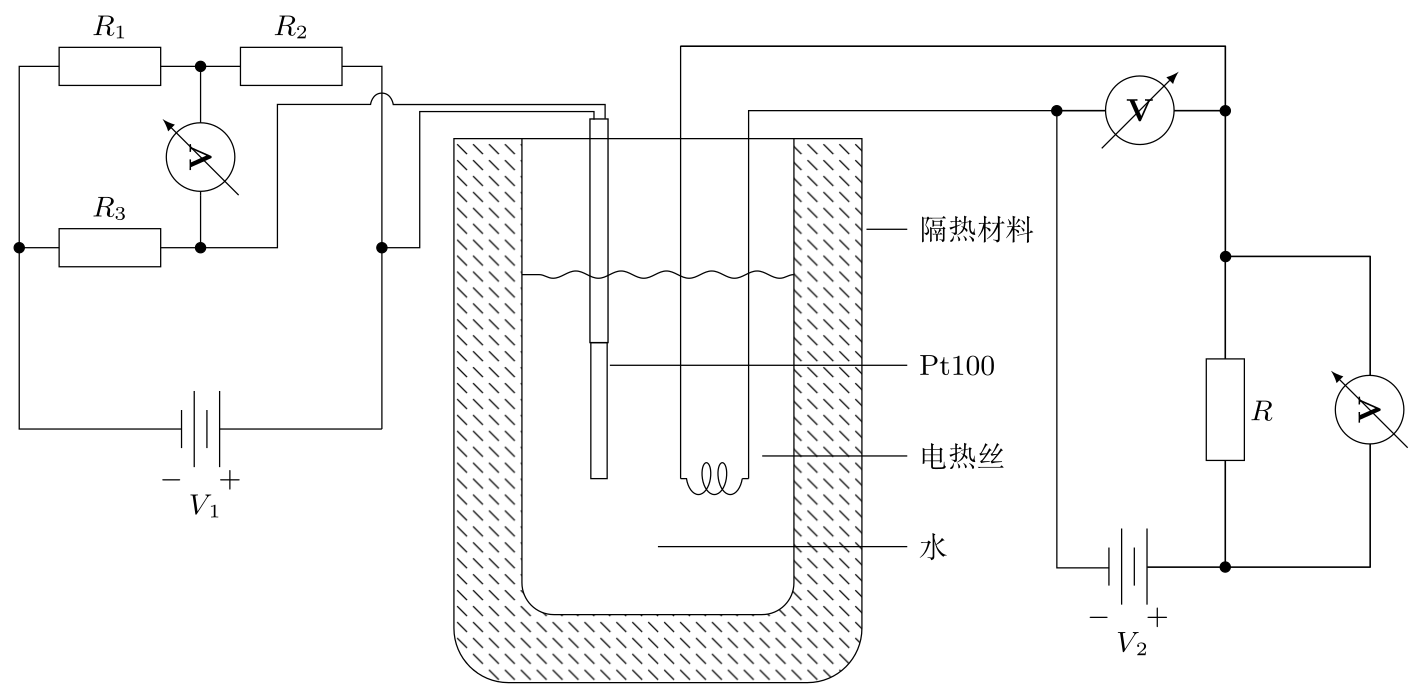
\includegraphics[width=.7\linewidth]{测量水比热/20240507200239.png}}
\caption[]{\label{fig:equi}仪器图}
\end{figure}
图中,左侧电路与 Pt100 作为自制温度计,通过电压表计算得出温度;右侧两个电压表分别用
于测量流经电热丝的电压与电流,用于计算功率。

\begin{table}[H]
  \caption[]{\label{tab:equi}仪器列表 }
\centering
% \vspace{4mm}
  \begin{longtable}{ll}
    \hline
    仪器 & 用途 \\
    \hline
    550 接口&数据采集处理\\
    计算机和 PASCO Capstone&数据采集平台、数据处理\\
    标准温度传感器&测温度\\
    电压传感器&测电压\\
    Pt100&自制温度传感器\\
    PN 结&自制温度传感器\\
    金属热电阻&自制温度传感器\\
    1Ω 电阻&与电压表结合作电流表\\
    100Ω 电阻&电桥电阻\\
    1000Ω 电阻&恒电流法电阻\\
    恒流恒压源&在恒流测量时获取恒流\\
    可调电源&获取可变功率\\
    温度传感实验装置&给温度传感器升温/降温\\
    保温容器&防止热量散失\\
    加热丝&给容器加热\\
    \hline
\end{longtable}
\end{table}
\longLine
\section{实验内容及具体步骤}
\begin{enumerate}
\item 第一步:了解敏感元件的温度特性
\item 第二步:测量随温度变化的物理量X
\item 第三步:利用T-X的关系和Capstone设计温度传感器
\item 第四步:将温度传感器用于测量其他物理量
\end{enumerate}

\subsection{Pt100 的温度-电阻特性}
1. 接线
2. 将 Pt100 放入温度传感实验装置内,给容器升温,使用 Pasco 550 测得温度与电压关系
3. 计算出温度与电阻关系并拟合

\subsection{测量金属热电阻的温度-电阻特性}
1. 接线
2. 调整电流大小至 VR1 为 0.1V ,此时当 R1 = 1000Ω 时,有电流 I = 100µA
3. 将金属热电阻放入温度传感实验装置内,给容器升温,使用 Pasco 550 测得温度与电压关系
4. 计算出温度与电阻关系并拟合
\subsection{由自制温度传感器测得水的比热容}
1. 称量铝容器的质量,装水,称量装水后质量2. 接线
3. 使用电热丝升温,记录电压、电流与自制温度计电压数据,计算出温度
4. 计算出水的比热容
\longLine
\section{数据记录及数据处理}
通过实验数据,作出图像
\subsection{Pt100}
\paragraph{升温}
获得拟合曲线为 $y=0.0058x+0.5659,R^2=0.9993$ 如图 \ref{fig:pt100up}
\paragraph{降温}
获得拟合曲线为 $y=0.0058x+0.5659,R^2=0.9993$ 如图 \ref{fig:pt100dn}
\begin{figure}[H]
\centering
\begin{subfigure}{.5\textwidth}
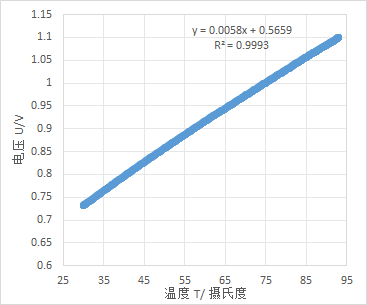
\includegraphics[width=.8\linewidth]{测量水比热/20240508101831.png}
\caption{\label{fig:pt100up} Pt100升温拟合}
\end{subfigure}\hfil
\begin{subfigure}{.5\textwidth}
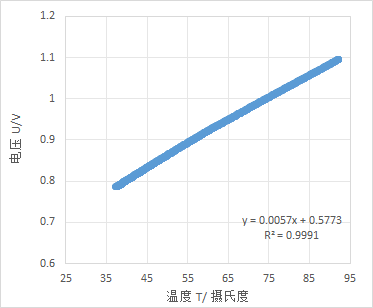
\includegraphics[width=.8\linewidth]{测量水比热/20240508104102.png}
\caption{\label{fig:pt100dn} Pt100降温拟合}
\end{subfigure}
\end{figure}


\subsection{PTC 温度特性}
\paragraph{升温}后期光滑,初期不平缓,拟合曲线为 $y=0.00003x^2-0.00305x+0.08155,R^2=0.92608$ 
\begin{figure}[H]
\centering
\begin{subfigure}{.5\textwidth}
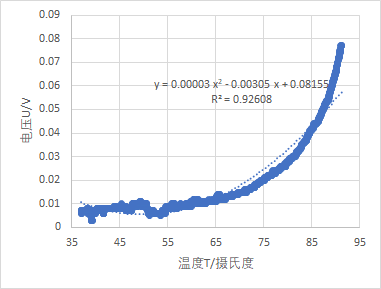
\includegraphics[width=.8\linewidth]{测量水比热/20240508111016.png}
\caption{\label{fig:pnup} PTC升温}
\end{subfigure}\hfil
\begin{subfigure}{.5\textwidth}
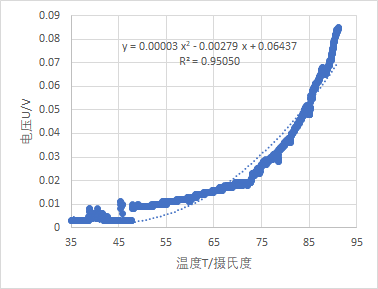
\includegraphics[width=.8\linewidth]{测量水比热/20240508111036.png}
\caption{\label{fig:pndn} PTC降温}
\end{subfigure}
\end{figure}
\paragraph{降温}和升温曲线相似,拟合曲线为 $y=0.00003x^3-0.00279x+0.06437,R^2=0.9505$ 
\subsection{PN 结温度特性}
\paragraph{升温}获得图像,注意到中间有突变,断裂,直接,拟合曲线为 $y=-0.0014x+0.5755,R^2=0.9845$ 如果分段拟合,斜率近似为 -0.0015 如图 \ref{fig:pt100up}
\begin{figure}[H]
\centering
\begin{subfigure}{.5\textwidth}
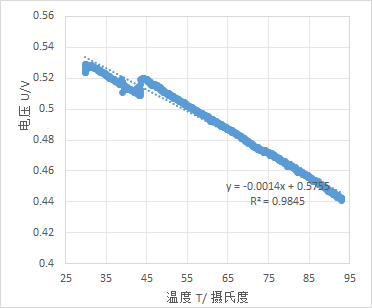
\includegraphics[width=.8\linewidth]{测量水比热/20240508104639.png}
\caption[]{\label{fig:pnup} PN 结升温}
\end{subfigure}\hfil
\begin{subfigure}{.5\textwidth}
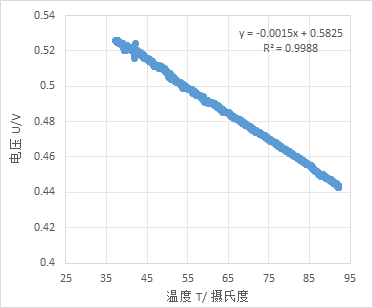
\includegraphics[width=.8\linewidth]{测量水比热/20240508105657.png}
\caption[]{\label{fig:pndn} PN 结降温}
\end{subfigure}
\end{figure}
\paragraph{降温}降温曲线没有突变,拟合曲线为 $y=-0.0015x+0.5825,R^2=0.9988$ 与之前一致。

\subsection{电阻特性计算}
利用电路结构,计算出电阻得到其它理论参数的数值。

Pt100 使用电桥法 $R=R_0 \frac{V+2V_x}{V-2V_x}$

PTC 使用恒电流法 $R=\frac{V_x}{I}$

PN 结使用恒电压法 $R=\frac{R_0}{V}-R$

将计算结果再次拟合作出:
\begin{figure}[H]
  \centering
  \begin{subfigure}{.3\textwidth}
    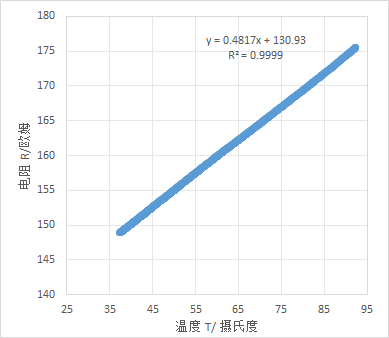
\includegraphics[width=\linewidth]{测量水比热/20240508122746.png}
    \caption{\label{fig:pt100R} Pt100 电阻与温度}
  \end{subfigure}\hfil
  \begin{subfigure}{.3\textwidth}
    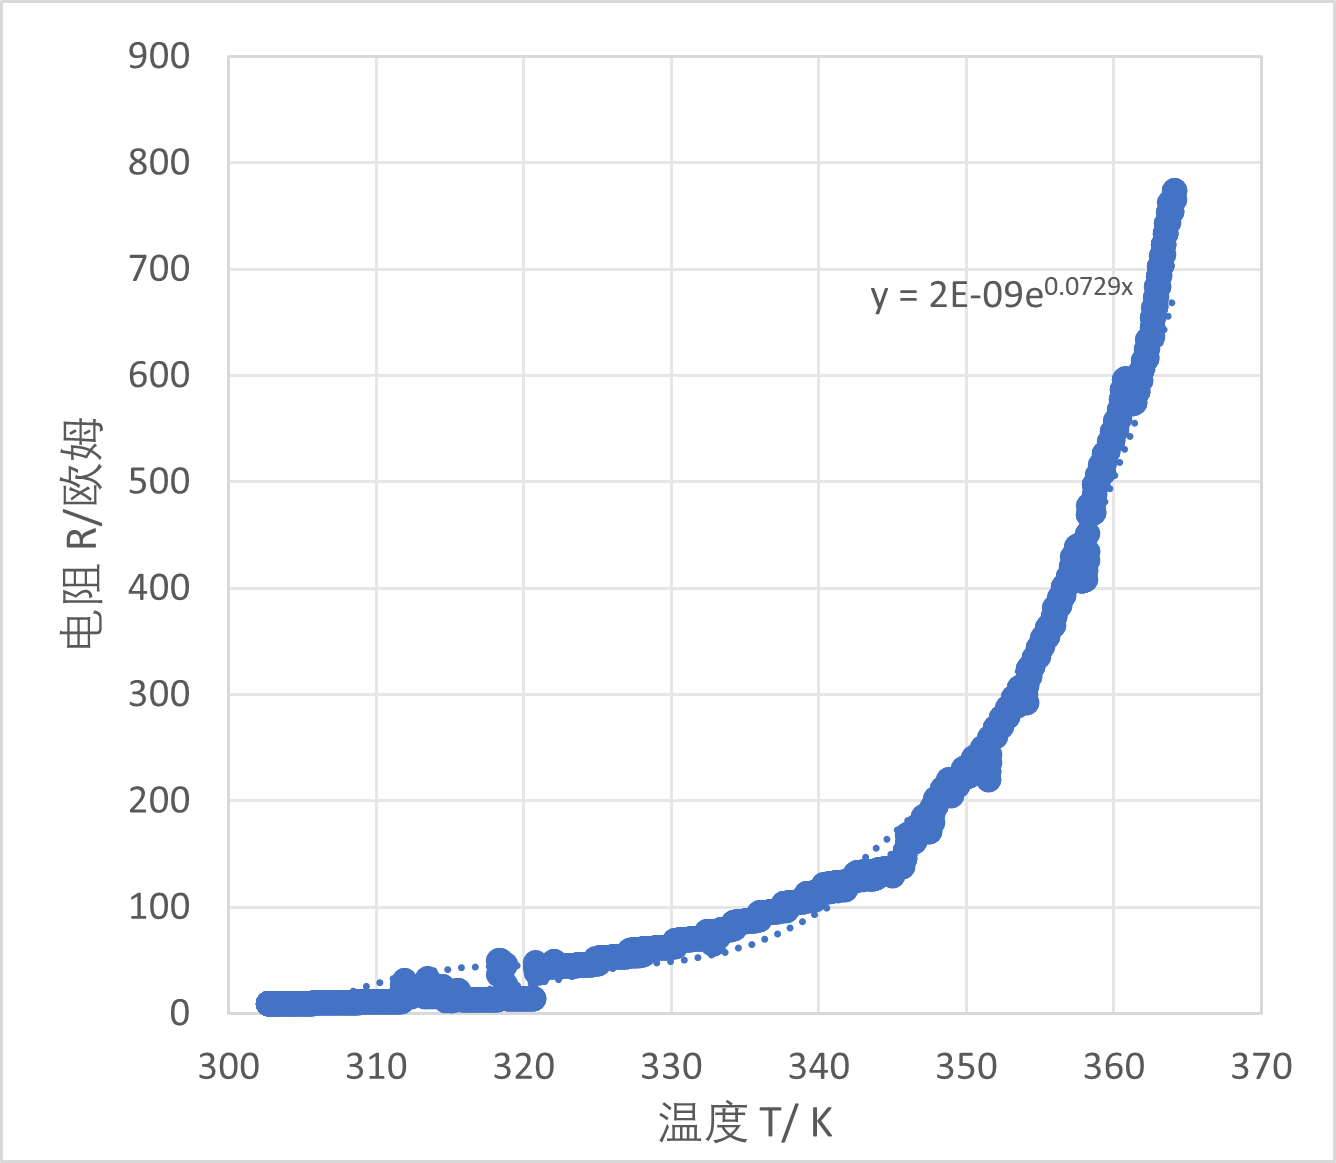
\includegraphics[width=\linewidth]{测量水比热/PTC.png}
    \caption[]{\label{fig:pnR} PTC 电阻与温度}
  \end{subfigure}\hfil
\begin{subfigure}{.3\textwidth}
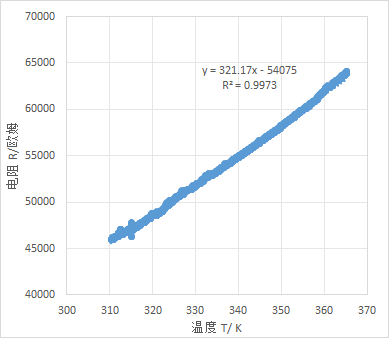
\includegraphics[width=\linewidth]{测量水比热/20240508152249.png}
\caption[]{\label{fig:pnR} PN 结电阻与温度}
\end{subfigure}
\end{figure}

总结其中的拟合结果,汇总特性到下表:
\begin{table}[H]
  \centering
\caption{不同温度传感器结果总结}
\begin{tabular}{lll}
  \hline
  器件 & 参数方程 & $R^2$ \\
  \hline
  Pt100 & y = 0.4817x + 130.93 & 0.9999 \\
  PTC & y = $2\times10^{-9}\mathrm{e}^{0.0729x}$ & 0.9908 \\
PN & y = 321.17x - 54075 & 0.9973 \\
  \hline
\end{tabular}
\end{table}

\subsubsection{误差分析}
参考 Pt100 温度系数 $3.85 × 10^{−3} /\textcelsius$ 计算上述结果和误差
\begin{gather}
\label{eq:12}
A=0.4817/130.93=3.6801 × 10^{−3} //\textcelsius\\
\varepsilon=|\frac{3.85-3.6801}{3.85}|\times100\%=4.41\%
\end{gather}

此误差在可接受范围之内。其它如PTC效果不好,
误差的因素有环境温度不稳定、电桥平衡电阻不精确、半导体材料不稳定、热敏电阻存在材料非线性响应等等。
\subsection{水的比热}
使用较方便的 Pt100 作自制温度计,加热过程中
使用软件积分功能,得到结果。
\begin{equation}
\label{eq:10}
\begin{split}
  I=V_2\cdot1\Omega\\
  P=V_2I \\
  \Delta W=\int P \mathrm{d}t
\end{split}
\end{equation}

已知铝比热 0.897 J/g/$\textcelsius$, 测得铝外壳质量 31 g。
测得水质量0.162 kg.
\begin{equation}
\label{eq:11}
\Delta \frac{W}{T}_{\text{Al}}=c_{\text{Al}}m=0.897\times31=27.807\text{ J/}\textcelsius
\end{equation}
使用之前实验的对照,可知初始温度 24$\textcelsius$ ,结束温度 48.17$\textcelsius$ ,结束时软件积分功率得到 $\Delta W=$ 19659.07

\begin{gather}
\label{eq:8}
\Delta T=48.17-24=24.17\textcelsius\\
\Delta W/\Delta T=\frac{19659.07}{24.17}=813.3665701 \text{ J/}\textcelsius\\
\Delta \frac{W}{T}_{w}=\Delta \frac{W}{T}-\Delta \frac{W}{T}_{\text{Al}}=813.3665701-27.807=785.5595701\text{ J/}\textcelsius
\end{gather}

\begin{equation}
\label{eq:13}
c_w=\Delta \frac{W}{T}_{w}/m=\frac{785.5595701}{0.162}=4849.133149 J/(kg\cdot\textcelsius)
\end{equation}

\subsubsection{误差分析}
\paragraph{比热容误差}
水的比热容一般被认为是是 $4849J · kg^{−1} · K^{−1}$
\begin{equation}
\label{eq:9}
\varepsilon=\left| \frac{4849-4200}{4200} \right|\times100\%=15.4\%
\end{equation}
对于热学实验,考虑到外界环境复杂性,这个误差水平应当是可以接受。
\paragraph{误差改进}
可能导致误差的因素有与外界的热量交换、环境温度变化、取样水纯净度、温度计本身读温度不准等等。
\longLine
\section{实验结果陈述与总结}

\subsection{结果陈述}
在本次比热容测量实验中,测得三种不同的元件的温度-电阻曲线
,计算了 Pt100 曲线与参考值的相对误差,并使用 Pt100 作为自制温度传感器测定了水的比热容为 $c = 4849J · kg^{−1} · K^{−1} $,
该值与理论值 $c_0 = 4200J · kg−1 · K−1$ 存在 $15.4\%$ 偏差。
\subsection{实验总结}
这次实验综合利用各种仪器进行温度传感测量,感受它们特殊的原理,发现不同可使用传感器的场景差异。
我掌握了实验操作的基本技巧,并意识到这些技巧在物理测量中的应用。尽管实验结果并未完全符合理论值,但通过对保温容器不绝热性的误差进行分析,我们认识到实验环境和设备性能对结果的重要影响。我学到了使用恒电流法和直流电桥法来测量热电阻,以及如何测量铂电阻和热敏电阻温度传感器的温度特性,还学到了如何测量PN结温度传感器的温度特性,以及如何利用自制温度传感器来测量水的比热容。
\endBox
\end{document}